\iffalse
\chapter{2021}
\section{ce}
\author{EE24BTECH11030}
\fi
\item The shape of the most commonly designed highway vertical curve is
\begin{enumerate}
\item circular (single radius)
\item circular (multiple radii)
\item parabolic
\item spiral
\end{enumerate}

\item A highway designed for 80 km/h speed has a horizontal curve section with radius 250 m. If the design lateral friction is assumed to develop fully, the required super elevation is
\begin{enumerate}
\item 0.02
\item 0.05
\item 0.07
\item 0.09
\end{enumerate} 

\item Which of the following is NOT a correct statement?
\begin{enumerate}
\item The first reading from a level station is a 'Fore Sight'.
\item Basic principle of surveying is to work from whole to parts.
\item Contours of different elevations may intersect each other in case of an overhanging cliff.
\item Planimeter is used for measuring 'area'.
\end{enumerate}


\item Which of the following is/are correct statement(s)?
\begin{enumerate}
\item Back Bearing of a line is equal to Fore Bearing $  180^\circ$.
\item If the whole circle bearing of a line is 270$^\circ$, its reduced bearing is 90$^\circ$ NW.
\item The boundary of water of a calm water pond will represent contour line.
\item In the case of fixed hair stadia tachometry, the staff intercept will be larger, when the staff is held nearer to the observation point.
\end{enumerate}

\bigskip
\item Consider the limit:
$[ \lim_{x \to 1} \left(\frac{1}{\ln x} - \frac{1}{x-1}\right) ]$
The limit (correct up to one decimal place) is$\underline{\hspace{2cm}}$.

\bigskip
\item The volume determined from $\int\int\int_{V}$
 8xyzdV for $V=[2,3]\times[1,2]\times[0,1]$ will be (in integer)$\underline{\hspace{2cm}}$

\bigskip
\item The state of stress in a deformable body is shown in the figure. Consider the transformation of the stress from the x-y coordinate system to the X-Y coordinate system. The angle $\theta$, locating the X-axis, is assumed to be positive when measured from the x-axis in the counter-clockwise direction. 
\begin{tikzpicture}

  % Axes
 \draw[->, thick] (0,0) -- (4,0) node[right] {$x$};
  \draw[->, thick] (0,0) -- (0,4) node[above] {$y$};
  % Dotted axes at 45 degrees
  \draw[dotted, thick] (0,0) -- (3,3) node[right] {$X$};
  \draw[dotted, thick] (0,0) -- (-3,3) node[left] {$Y$};
  % Half arrow pointing downwards to the left of the y-axis
  \draw[-{Straight Barb[right]}, thick] (-0.2,2) -- (-0.2,0.5);
  \draw[-{Straight Barb[left]}, thick] (1.7,-0.2) -- (0.2,-0.2);
  \draw[-{Straight Barb[left]}, thick] (0.5,1.8) -- (1.75,0.95)node[right] {$\sigma_{xx} = 50 \text{ MPa}$};
  % Left arrow with label just above it
  \draw[->, thick] (-0.3,1.65) -- (-1.2,1.65) 
     node[above] {$\sigma_{xx} = 40 \text{ MPa}$};
  % Triangle
  \draw[thick] (0,0) -- (3,0) -- (0,2) -- cycle;
  % Labels
  \draw[thick,->] (2.5,0) arc[start angle=180, end angle=150, radius=0.5cm];
  % Label the angle
  \node at (2, 0.2) {$30^\circ$};
  % Stress components
  \draw[->, thick] (1.3,1.3) -- (2.3,2.3) node[right] {$\sigma_{xx} = 120 \text{ MPa}$};
 \draw[->, thick] (0.5,-0.22) -- (0.5,-1.22) node[below] {$\sigma_{yy} = 35.6 \text{ MPa}$};
 % Adjust arrowhead size and line thickness as needed
 \tikzset{>=latex} % Adjust arrowhead style

\end{tikzpicture}

The absolute magnitude of the shear stress component $\sigma_{xy}$ (in MPa, round off to one decimal place) in the x-y coordinate system is$\underline{\hspace{2cm}}$
\bigskip
\item The equation of deformation is derived to be $y=x^2 - xL$ for a beam shown in the figure $\ref{fig:fig-8}$.
\begin{figure}[h] % 'h' means place the figure here
    \centering
    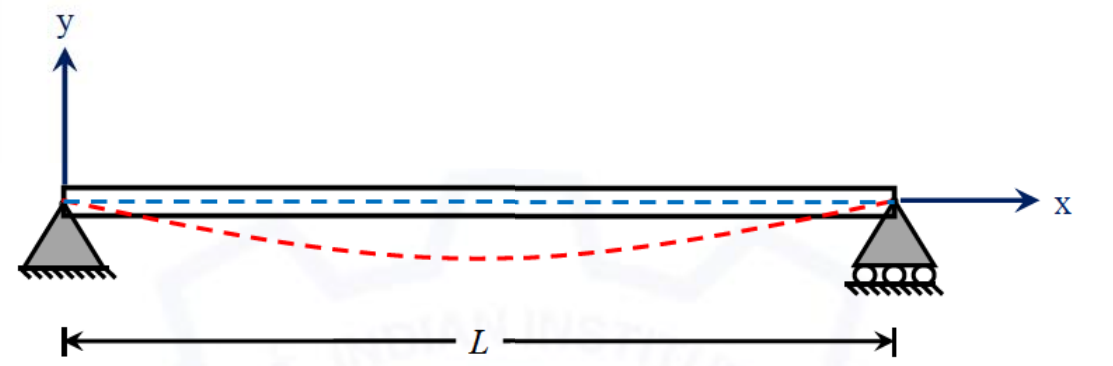
\includegraphics[width=\textwidth]{GATE-yearwise/GATE(10)/figs/fig1.png}
    \caption{}
    \label{fig:fig-8}
\end{figure}
\\The curvature of the beam at the mid-span(in units,in integer) will be $\underline{\hspace{2cm}}$
\bigskip
\item A truss EFGH is shown in the figure, in which all the members have the same axial rigidity R. In the figure, P is the magnitude of external horizontal forces acting at joints F and G.
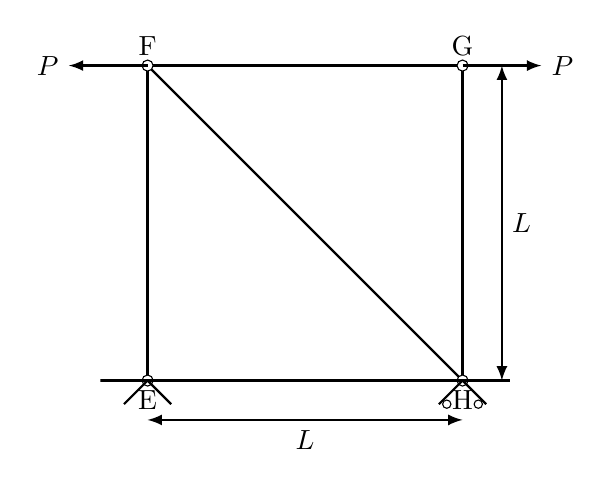
\begin{tikzpicture}

    % Define coordinates for the nodes
    \coordinate (F) at (0,0);
    \coordinate (G) at (4,0);
    \coordinate (E) at (0,-4);
    \coordinate (H) at (4,-4);

    % Draw the truss members
    \draw[thick] (F) -- (G) -- (H) -- (E) -- cycle;
    \draw[thick] (F) -- (H);

    % Add small circles for vertices
    \filldraw[fill=white] (F) circle (2pt);
    \filldraw[fill=white] (G) circle (2pt);
    \filldraw[fill=white] (E) circle (2pt);
    \filldraw[fill=white] (H) circle (2pt);

    % Add labels
    \node[above] at (F) {F};
    \node[above] at (G) {G};
    \node[below] at (E) {E};
    \node[below] at (H) {H};

    % Add forces
    \draw[<-, thick] (-1, 0) -- (F) node[left=1cm] {$P$};
    \draw[->, thick] (G) -- (5,0) node[right] {$P$};

    % Add dimensions
    \draw[<->, thick] (0,-4.5) -- (4,-4.5) node[midway, below] {$L$};
    \draw[<->, thick] (4.5,0) -- (4.5,-4) node[midway, right] {$L$};

    % Fixed support at E
    \draw[thick] (E) -- ++(-0.3,-0.3);
    \draw[thick] (E) -- ++(0.3,-0.3);
    \draw[thick] (E) -- ++(-0.6,0) -- ++(1.2,0);

    % Roller support at H
    \draw[thick] (H) -- ++(-0.3,-0.3);
    \draw[thick] (H) -- ++(0.3,-0.3);
    \draw[thick] (H) -- ++(-0.6,0) -- ++(1.2,0);
    \draw (H) ++(-0.2,-0.3) circle (1.5pt);
    \draw (H) ++(0.2,-0.3) circle (1.5pt);

\end{tikzpicture}
If $R = 500\times 10^3$ kN, P = 150 kN, and L = 3m, the magnitude of the horizontal displacement of joint G (in mm, round off to one decimal place) is$\underline{\hspace{2cm}}$
\bigskip
\item The cohesion (c), angle of internal friction ($\phi$), and unit weight ($\sigma$) of a soil are 15 kPa, 20$^\circ$, and 17.5 kN/m$^3$, respectively. The maximum depth of unsupported excavation in the soil (in m, round off to two decimal places) is$\underline{\hspace{2cm}}$

\bigskip
\item Two reservoirs are connected through a homogeneous and isotropic aquifer having hydraulic conductivity (K) of 25 m/day and effective porosity ($\eta$) of 0.3 as shown in the figure (not to scale). Groundwater is flowing in the aquifer at the steady state. \\
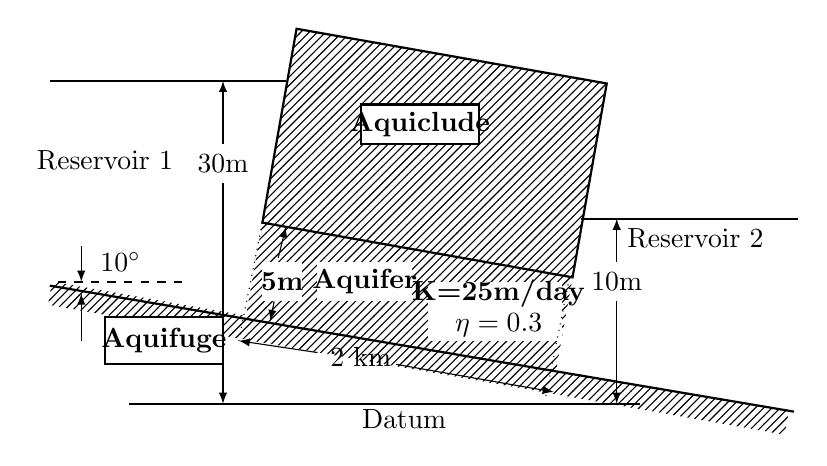
\begin{tikzpicture}
    % Define the angle of rotation for the main rectangle
    \usetikzlibrary{patterns}
    \begin{scope}[rotate=-10]
        % Draw and fill the main rectangle with a pattern
        \fill[pattern=north east lines] (0,0) rectangle (4,2.5);
        \draw[thick] (0,0) rectangle (4,2.5);
        \fill[pattern=north east lines] (0,0) rectangle (4,-1.2);
        \fill[pattern=north east lines] (-2.5,-1.2) rectangle (7,-1.5);
    \end{scope}
    
    % Draw a small horizontal white box inside the inclined rectangle (without rotation)
    \fill[white] (1.25,1) rectangle (2.75,1.5);
    \draw[thick] (1.25,1) rectangle (2.75,1.5);
    \fill[white] (-2,-1.2) rectangle (-0.5,-1.8);
    \draw[thick] (-2,-1.2) rectangle (-0.5,-1.8);
    \node at (-1.25,-1.5) {\textbf{Aquifuge}};
    % Add the text "Aquiclude" in bold font inside the small box
    \node at (2,1.25) {\textbf{Aquiclude}};

    \fill[white] (0,-1) rectangle (0.5,-0.5);
    \node at (0.25,-0.75) {\textbf{5m}};
    \draw[->] (0.2,-0.45) -- (0.3,-0.05);
    \draw[->] (0.15,-1) -- (0.1,-1.25);
    \fill[white] (0.7,-0.5) rectangle (1.9,-1);
    \node at (1.3,-0.75) {\textbf{Aquifer}};

    \fill[white] (2.1,-0.75) rectangle (3.8,-1.5);
    \node at (3,-0.9) {\textbf{K=25m/day}};
    \node at (3,-1.3) {\textbf{$\eta=0.3$}};
    % Draw a horizontal line 3 cm to the left of the inclined rectangle
    \draw[thick] (-2.7,1.8) -- (0.3,1.8);
    \draw[thick] (4.05,0.05) -- (6.8,0.05);
    \draw[thick] (-1.7,-2.3) -- (4.8,-2.3);
    \node at (1.8,-2.5) {Datum};
    \draw[thick] (-2.7,-0.8) -- (6.75,-2.4);
    \draw[->] (-0.5,1) -- (-0.5,1.8);
    \node at (-0.5,0.75) {30m};
    \node at (-2,0.8) {Reservoir 1};
    \draw[->] (-0.5,0.5) -- (-0.5,-2.3);
    \draw[->] (4.5,-0.5) -- (4.5,0.05);
    \node at (4.5,-0.75) {10m};
    \node at (5.5,-0.2) {Reservoir 2};
    \draw[->] (4.5,-1) -- (4.5,-2.3) ;
    
    \draw[->] (0.7,-1.65) -- (-0.3,-1.5);
    \node at (1.25,-1.7) {2 km};
    \draw[->] (1.7,-1.8) -- (3.7,-2.15) ;
    
    % Draw dotted lines parallel to the larger rectangle, 2 cm below
    \draw[dotted] (0, 0) -- (-0.3, -1.5);
    \draw[dotted] (3.9, -0.7) -- (3.6, -2.2);
    \draw[dashed, thick] (-2.6,-0.75) -- (-1,-0.75) ;
    \draw[->] (-2.3,-0.3) -- (-2.3,-0.75);
    \node at (-1.8,-0.5) {$10^{\circ}$};
    \draw[->] (-2.3,-1.5) -- (-2.3,-0.9) ;

\end{tikzpicture}

If water in Reservoir 1 is contaminated, then the time (in days, round off to one decimal place) taken by the contaminated water to reach  Reservoir 2 will be$\underline{\hspace{2cm}}$
\bigskip
\item A signalized intersection operates in two phases. The lost time is 3 seconds per phase. The maximum ratios of approach flow to saturation flow for the two phases are 0.37 and 0.40. The optimum cycle length using the Webster's method (in seconds, round off to one decimal place) is$\underline{\hspace{2cm}}$
\bigskip
    \item The solution of the second-order differential equation 
    \[
    \frac{d^2 y}{dx^2} + 2 \frac{dy}{dx} + y = 0
    \]
    with boundary conditions $y(0) = 1$ and $y(1) = 3$ is
    \begin{enumerate}
        \item $e^{-x} + (3e - 1) x e^{-x}$
        \item $e^{-x} - (3e - 1) x e^{-x}$
        \item $e^{-x} + \left[ 3 \sin \left( \frac{\pi x}{2} \right) - 1 \right] x e^{-x}$
        \item $e^{-x} - \left[ 3 \sin \left( \frac{\pi x}{2} \right) - 1 \right] x e^{-x}$
    \end{enumerate}

